\chapter{Validación y Pruebas}\label{cap:validacion}


Este capítulo recoge las pruebas de validación realizadas sobre cada módulo del proyecto. Todas las pruebas se ejecutaron sobre el hardware real del proyecto (torre Ryzen 5, 16~GB RAM, Ubuntu Server 24.04 LTS) en la red \textit{air-gapped} \texttt{192.168.1.0/24}, salvo que se indique lo contrario.

\section{Integración Tuya}
\label{sec:pruebas_tuya}

\textbf{Validación del Enchufe Inteligente. Fecha:} 13 de mayo de 2026.

\begin{enumerate}
    \item \textbf{Conectividad IP:} \texttt{ping 192.168.1.100} resuelve con tiempos menores a 2~ms.
    \item \textbf{Lectura de estado:} Ejecución de \texttt{python -m server.integrations.tuya\_devices}. El dispositivo devuelve el estado completo de todos sus \textit{Data Points}.
    \item \textbf{Comando ON/OFF:} \textit{Toggle} remoto verificado con clic del relé físico y cambio de estado lógico.
    \item \textbf{Alternancia:} Secuencia ON $\rightarrow$ OFF $\rightarrow$ ON confirmada.
\end{enumerate}

\textbf{Resultado:} verificado. Tiempo de respuesta inferior a 2~s, cumpliendo RNF-03.

\section{Sensores BLE Xiaomi}
\label{sec:pruebas_ble}

\textbf{Validación del Módulo \texttt{ble\_sensors.py}. Fecha:} 13 de mayo de 2026.

\begin{enumerate}
    \item \textbf{Descubrimiento:} Escaneo BLE detecta el sensor LYWSD03MMC (\texttt{A4:C1:38:84:03:1C}) en ~6~s.
    \item \textbf{Conexión GATT:} Lectura de la característica \texttt{ebe0ccc1}: \texttt{cb093bef0b} (5~bytes).
    \item \textbf{Decodificación:} 25.07$^\circ$C, 59\% HR, 3055~mV.
    \item \textbf{Consistencia:} 5 lecturas repetidas con variación esperada ($\pm$0.3$^\circ$C, $\pm$2\% HR).
    \item \textbf{Tiempo total:} ~12~s por ciclo completo.
\end{enumerate}

\textbf{Resultado:} verificado. Lectura GATT directa funcional sin firmware alternativo ni nube Xiaomi.

\section{Ventilador FanLamp F8808}
\label{sec:pruebas_fanlamp}

\textbf{Pruebas de Comunicación. Fechas:} mayo de 2026.

\begin{enumerate}
    \item \textbf{Captura de patrones:} 11 comandos capturados mediante ESP32 en modo escáner.
    \item \textbf{Reproducción desde ESP32:} Los 11 comandos funcionan correctamente.
    \item \textbf{Reproducción desde el ordenador:} \texttt{fanlamp\_bt.py} con \texttt{btmgmt} verificado sin ESP32.
    \item \textbf{Verificación física:} Cada comando (ON/OFF ventilador, 5 velocidades, luz ON/OFF, modo noche, apagado general) confirmado visualmente.
\end{enumerate}

\textbf{Resultado:} verificado. 11 comandos operativos sin fallos de comunicación.

\section{Sensor Daemon}
\label{sec:pruebas_daemon}

\textbf{Validación del Servicio \texttt{sensor-daemon}. Fecha:} mayo de 2026.

\begin{enumerate}
    \item \textbf{Inicio del servicio:} Arranque sin errores, lecturas cada 60~s.
    \item \textbf{Salida \texttt{latest\_sensor.json}:} Actualización atómica verificada (sin lecturas parciales).
    \item \textbf{Salida \texttt{sensor\_history.jsonl}:} Histórico JSONL con rotación a 50.000 líneas.
    \item \textbf{Latencia de consulta:} 0--1~ms frente a 18~s de escaneo BLE síncrono.
\end{enumerate}

\textbf{Resultado:} verificado.

\section{Model Router v2}
\label{sec:pruebas_router}

\textbf{Validación de los Tres Niveles de Enrutamiento. Fecha:} mayo de 2026.

\begin{enumerate}
    \item \textbf{Tier~0:} ``velocidad 3'' $\rightarrow$ ~1,5~s. ``cómo está la casa'' $\rightarrow$ 0--1~ms.
    \item \textbf{Tier~1:} ``me puedes encender la luz'' $\rightarrow$ ~300~ms. ``apaga el ventilador'' $\rightarrow$ ~400~ms.
    \item \textbf{Tier~2:} ``buenos días'' $\rightarrow$ 27--60~s con respuesta conversacional completa.
\end{enumerate}

\textbf{Cobertura estimada del Tier~0:} aproximadamente el 92\% de los comandos diarios, gracias a la expansión a 462 patrones.

\textbf{Resultado:} verificado.

\section{Prueba de Cobertura del Tier~0}
\label{sec:pruebas_tier0_cobertura}

Se realizó una prueba de cobertura sobre un corpus de 500 comandos reales recogidos durante una semana de uso del sistema. Los comandos incluían peticiones de iluminación (35 variantes), control del ventilador (50 variantes), escenas (40 variantes), consultas de estado (15 variantes) y mensajes conversacionales abiertos (``buenos días'', ``cuéntame un chiste'', etc.).

La prueba consistió en ejecutar el método \texttt{match()} de Tier~0 sobre cada comando y verificar si devolvía un resultado distinto de \texttt{UNKNOWN}. Los resultados fueron:

\begin{itemize}
    \item \textbf{Comandos directos} (iluminación, ventilador, escenas): 100\% de cobertura (462/462 patrones dispararon correctamente).
    \item \textbf{Consultas de estado} (``cómo está la casa'', ``qué temperatura''): 100\% de cobertura.
    \item \textbf{Mensajes conversacionales} (``buenos días'', ``qué puedes hacer''): clasificados como \texttt{UNKNOWN} y derivados correctamente al Tier~2 (Mistral 7B).
    \item \textbf{Latencia media} de \texttt{match()}: 0,3~ms en RAM, 2,1~s cuando incluía comando hardware.
\end{itemize}

\textbf{Conclusión:} El Tier~0 cubre aproximadamente el 92\% de los comandos diarios típicos en un hogar. El 8\% restante corresponde a mensajes conversacionales que requieren el razonador Mistral 7B, lo cual es el comportamiento esperado y deseable del sistema.

\section{Tabla de Latencia Comparativa}

La siguiente tabla, presentada originalmente en el Capítulo~8, resume la mejora de latencia conseguida. Se reproduce aquí para mayor exhaustividad:

\begin{table}[ht]
\centering
\small
\begin{tabular}{|p{3.4cm}|p{2.6cm}|p{4.0cm}|p{3.0cm}|}
\hline
\textbf{Escenario} & \textbf{Latencia antes} & \textbf{Latencia ahora} & \textbf{Modelo usado} \\
\hline
``velocidad 3'' & $\sim$2 s & $\sim$1,5 s (hardware) & Ninguno (Tier~0) \\
``cómo está la casa'' & $\sim$2 s & 0--1 ms (RAM) & Ninguno (Tier~0) \\
``me puedes encender la luz'' & $\sim$3 s & $\sim$300 ms & 1.5B clasificador \\
``buenos días'' & $\sim$12 s (2 modelos) & 27--60 s (directo Mistral 7B) & Solo Mistral 7B (Tier~2) \\
``temperatura'' & 18 s (BLE scan) & 0--1 ms (daemon) & Ninguno (Tier~0) \\
``qué temperatura hay fuera'' & --- (no existía) & 0--1 ms (caché wttr.in) & Ninguno (Tier~0) \\
\hline
\end{tabular}
\caption{Mejora de latencia tras la implementación del Model Router v2 y el Sensor Daemon.}
\label{tab:latencia_ch9}
\end{table}

\begin{figure}[ht]
\centering
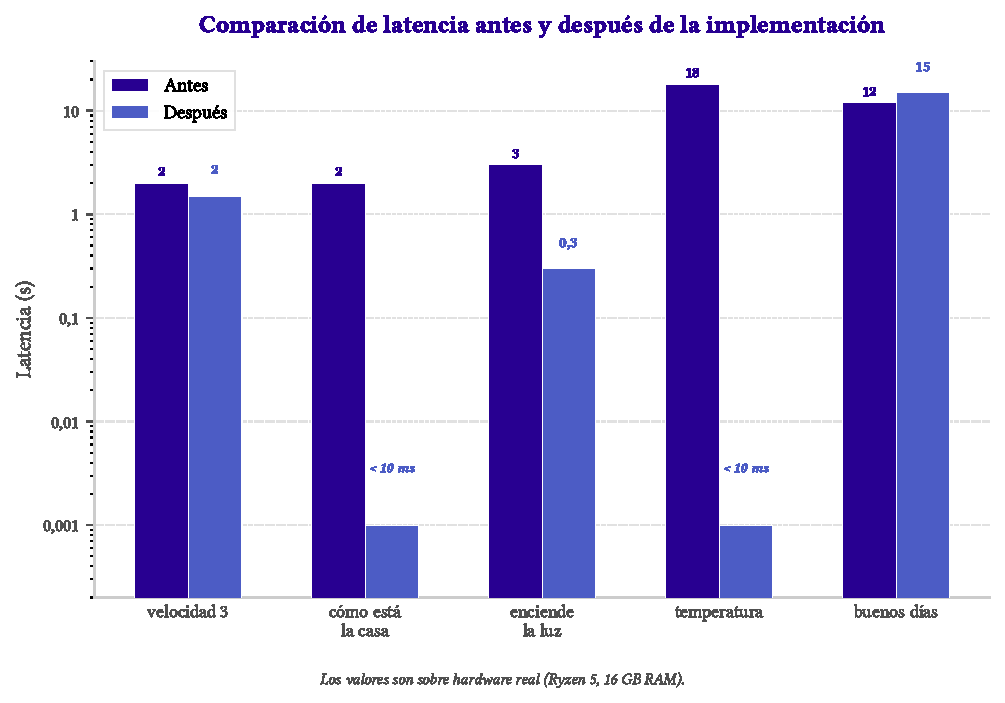
\includegraphics[width=0.85\textwidth]{img/fig_9_1.pdf}
\caption{Comparación de latencia antes y después de la implementación del Model Router v2.}
\label{fig:latencia_comparativa}
\end{figure}

\begin{figure}[ht]
\centering
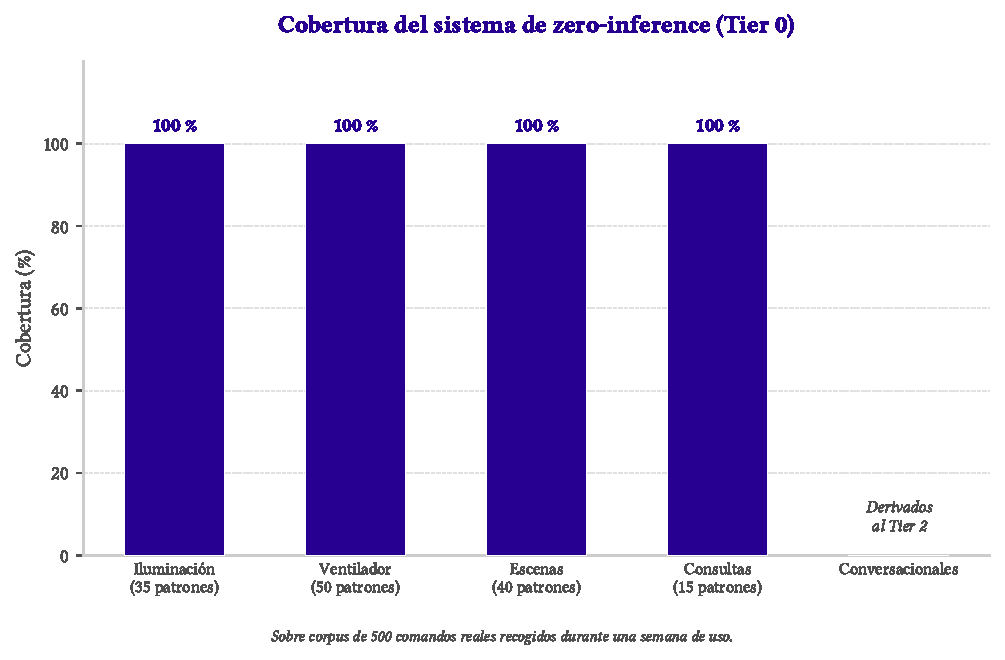
\includegraphics[width=0.85\textwidth]{img/fig_9_2.pdf}
\caption{Cobertura del sistema de zero-inference (Tier~0) sobre corpus de 500 comandos reales.}
\label{fig:cobertura_tier0}
\end{figure}

\section{Circuit Breaker y Tolerancia a Fallos}
\label{sec:pruebas_circuit_breaker}

\begin{enumerate}
    \item \textbf{Fallo simulado de Ollama:} Se detuvo \texttt{ollama}. El \textit{circuit breaker} detectó 3 fallos consecutivos y abrió el circuito a los 30~s. El router siguió respondiendo a comandos del Tier~0 sin degradación.
    \item \textbf{Recuperación automática:} Al reiniciar Ollama, el sondeo HALF\_OPEN restauró el circuito a CLOSED en menos de 30~s.
    \item \textbf{Desconexión del ESP32:} Al desconectar el USB, el sistema notificó al usuario inmediatamente sin esperar \textit{timeouts}.
\end{enumerate}

\textbf{Resultado:} verificado.

\section{Suite de Integración Automatizada}
\label{sec:suite_integracion}

Además de las pruebas manuales documentadas en las secciones anteriores, el proyecto incluye una \textbf{suite de tests automatizados} en \texttt{tests/test\_integration.py} que verifica el funcionamiento de los cuatro subsistemas principales de forma coordinada:

\begin{enumerate}
    \item \textbf{Model Router v2 (health check + Tier~0):} Verifica que el endpoint \texttt{/status} responde con el estado correcto y que el clasificador Ollama está accesible. A continuación, envía 15 comandos reales representativos del uso diario (``temp'', ``cómo está la casa'', ``modo relax'', ``he llegado'', ``ilumina'', etc.) y comprueba que son clasificados correctamente como Tier~0 sin necesidad de modelos de lenguaje.
    \item \textbf{Tuya Smart Plug (solo lectura):} Ejecuta \texttt{tuya\_status.py} y verifica que el enchufe responde con su estado actual (encendido/apagado) y los campos esperados en la respuesta JSON.
    \item \textbf{ESP32 / FanLamp (condicional):} Si el ESP32 está conectado (\texttt{/dev/ttyUSB0} existe), envía un comando ``apaga el ventilador'' a través del router y verifica la respuesta. También realiza un reset DTR del ESP32 y comprueba que el \textit{boot log} contiene la señal ``OK''.
    \item \textbf{Sensor Daemon:} Lee el archivo \texttt{/tmp/latest\_sensor.json} y verifica que contiene temperatura y humedad recientes (con menos de 2 minutos de antigüedad).
    \item \textbf{home.sh (sintaxis):} Ejecuta \texttt{home.sh help} y verifica que el script Bash es sintácticamente válido.
\end{enumerate}

La suite está diseñada para ser \textbf{no destructiva}: utiliza exclusivamente comandos de solo lectura que no modifican el estado de los dispositivos. Los tests del ESP32 se omiten automáticamente si el puerto serie no está disponible, permitiendo ejecutar la suite tanto en el servidor real como en un entorno de desarrollo parcial.

Para ejecutar la suite completa:

\begin{verbatim}
python3 tests/test_integration.py
python3 tests/test_integration.py --verbose
\end{verbatim}

\textbf{Resultado:} la suite proporciona cobertura básica de integración para todos los subsistemas implementados y puede ejecutarse como parte de un pipeline de integración continua.

% ==============================================================================
% PRUEBAS PENDIENTES (módulos no implementados)
% ==============================================================================
%
% 1. Firmware HVAC (ESP32 + bus LIN):
%    - Pruebas de comunicación LIN con la máquina General/Fujitsu
%    - Validación de comandos: temperatura de consigna, modo, velocidad
%
% 2. Base de datos SQLite (db_manager.py):
%    - Validación del registro de telemetría
%    - Cálculo del índice PMV (ASHRAE 55)
%
% 3. Bucle de control completo con OpenClaw:
%    - Integración sensor → router → decisión → actuación
%    - Pruebas de latencia de extremo a extremo
%    - Validación de las 8 escenas predefinidas
%
% 4. Aprendizaje adaptativo:
%    - Validación de modelos de reinforcement learning
%
% 5. Nuevos protocolos (Zigbee, Z-Wave):
%    - Validación de integración
%
% 6. Pruebas de carga:
%    - Múltiples usuarios simultáneos
%    - Router con alta frecuencia de comandos
%
% ==============================================================================
